\section{Электроинструмент}

\clearpage
\subsection{Дрелъ}

\noindent
\begin{tabular}{p{0.5\textwidth} p{0.5\textwidth}}
\noindent
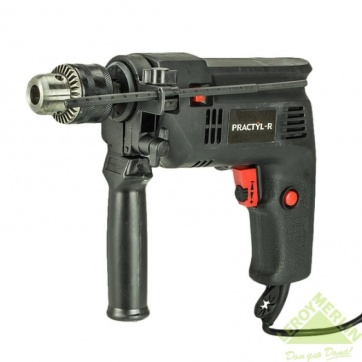
\includegraphics[width=0.45\textwidth]{tech/tools/PraktylR.jpg}
&
\noindent
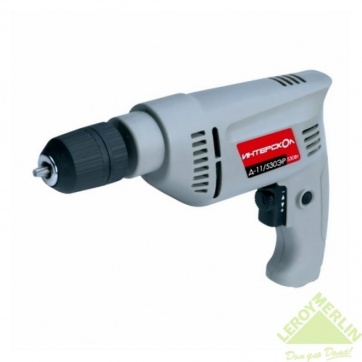
\includegraphics[width=0.45\textwidth]{tech/tools/D_11_530ER.jpg}
\\
\textbf{Дрель ударная сетевая} & \textbf{Дрель безударная сетевая} \\
\textbf{Praktyl-R PID13D01 400\,Вт} 
\href{http://leroymerlin.ru/catalogue/instrumenty/elektroinstrument/dreli\_udarnye/13805983/}{\textbf{(!)395\,р.}}
&
\textbf{Интерскол Д-11/530ЭР (с БЗП)}
\href{http://leroymerlin.ru/catalogue/instrumenty/elektroinstrument/dreli\_bezudarnye/11857763/}{\textbf{1120\,р.}}
\\
\end{tabular}
\bigskip

Дрель\ --- одноразовая китайчатина от 400\,р. Продаются уже брендированные на
Леруа Мерлен, наклейка <<PID13D01 Ударная дрель 400\,Вт, 13\,мм>>. Скорость
регулируется глубиной нажатия курка, крутилка на курке ограничивает глубину
механически, фиксатор держит скорость близко к минимальной, запаха горелой
пластмассы через несколько минут работы на холостом ходу нет.

По надежности рекомедуется Интерскол 1100+\,р. Надежность Интерскола\ --- не
<<китай>>, классика ДУ-580ЭР работает в хвост и гриву, используется криворукими
студентами, лежит в подвале в пыли от точила, и никаких вопросов даже со
щетками.

Если не планируете много сверлить бетон, \textbf{берите дрель без ударного
механизма}: отсутствуют лишние продольные перемещения, что может быть важно при
использовании в качестве шпинделя сверлильного станка, и механизации других
технологических поделок.

У шуруповерта нет 43\,мм шейки для фиксации, поэтому как средство электропривода
он практически бесполезен, и нужен собственно для заворачивания большого
количества саморезов. Хотя наличие ограничителя крутящего момента и малые
габариты удобны при сверлении и сборке поделок.

\bigskip
Имея некоторое количество поделочного материала, кривые руки и особенно доступ к
станочному оборудованию, можно сколкозить некоторое подобие настольных
станочков\ \pref{fig:drelstans}\ для механизации некоторых работ,
используя дрель в качестве привода.

Главным элементом такой оснастки\ --- зажим на шейку дрели 43\,мм. Особых
требований по его точности и качеству нет, т.к. сама шейка обычно пластиковая, и
никакой доводки по круглости и параллельности оси инструмента не проходит.

\clearpage
\phantomsection\label{fig:drelstans}
\noindent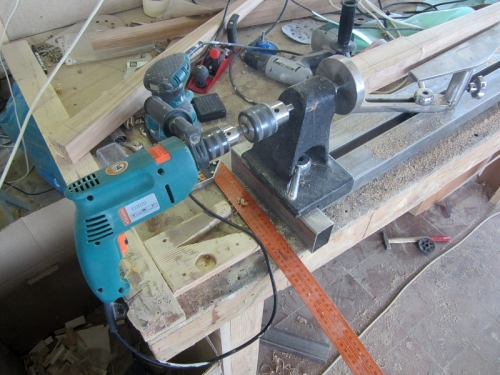
\includegraphics[height=0.528\textheight]{tech/tools/DrelLathe.jpg}
\noindent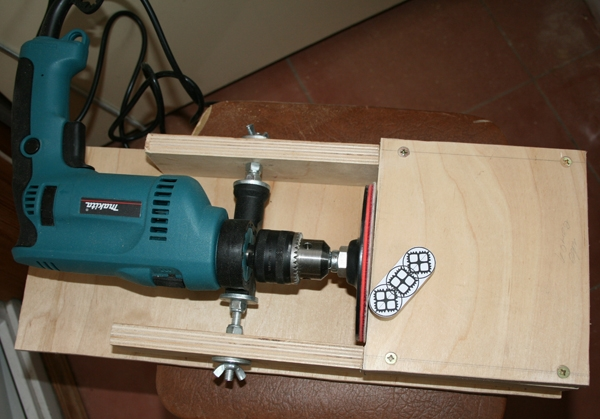
\includegraphics[height=0.528\textheight]{tech/tools/DrelShliph.jpg}

\noindent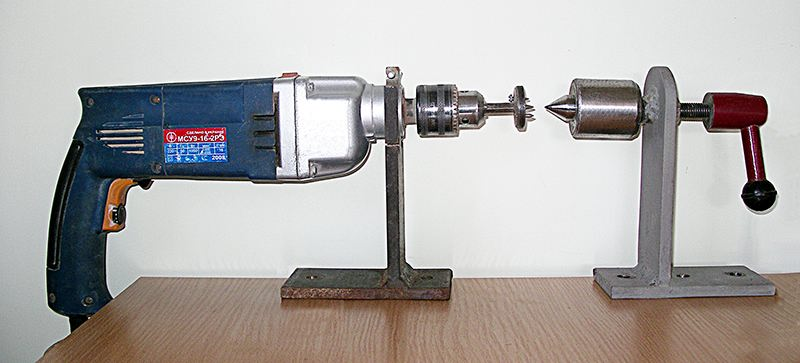
\includegraphics[height=0.465\textheight]{tech/tools/DrelLathe2.jpg}
\noindent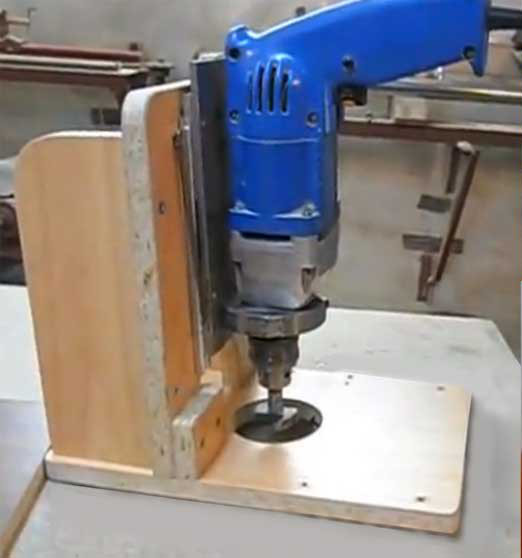
\includegraphics[height=0.465\textheight]{tech/tools/DrelBoren.jpg}
\clearpage

\subsection{Лобзик}

\noindent
\begin{tabular}{p{0.5\textwidth} p{0.5\textwidth}}
\noindent
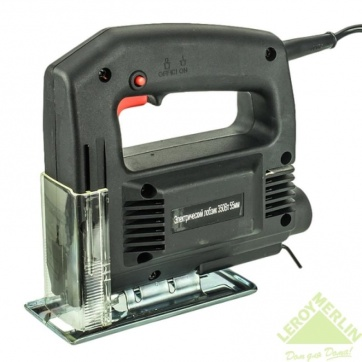
\includegraphics[width=0.45\textwidth]{tech/tools/LobzPraktyl.jpg}
&
\noindent
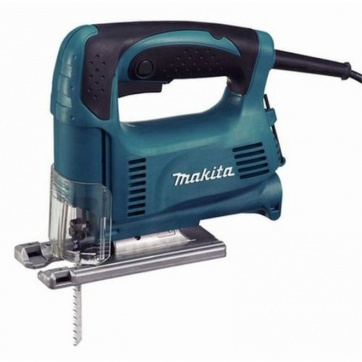
\includegraphics[width=0.45\textwidth]{tech/tools/LobzMakita4329.jpg}
\\
\href{http://leroymerlin.ru/catalogue/instrumenty/elektroinstrument/lobziki/13805991/}{\textbf{Praktyl
350 Вт 356\,р.}} 
& 
\href{http://leroymerlin.ru/catalogue/instrumenty/elektroinstrument/lobziki/12114283/}{\textbf{Makita
4329 2260\,р.}}
\\
\end{tabular}
\bigskip

Лобзик полезен при разделке стеклотекстолита, и изготовлении технологической
мебели (стеллажи, рабочие столы и т.п.).

\subsection{Жвигатель}

Если у вас возникло желание механизировать изготовление механических деталей, а
свободного доступа к настоящему станочному оборудованию нет, есть смысл
рассмотреть изготовление самодельной механизированной оснастки 
типа\ \pref{fig:drelstans}, или даже самодельных станочков. В этом случае надо
рассмотреть применения универсального привода.

Первый кандидат на место универсального электропривода достается той самой
дрели, не забываем об обязательном наличии 43\,мм монтажной шейки.
Достоинство дрели как привода\ --- прямое подключение к сети, встроенный
редуктор, есть модели с простой регулировкой оборотов, есть резьба и отверстие
под винт на валу, в комплекте есть патрон для зажима мелких деталей в
точилке\footnote{\ БЗП удобен, патрон с ключем дает лучший зажим и возможно
точнее}.

Ограниченно доставаемые двигатели от стиральных машин, отличаются мощностю и
оборотистостью, особенно от старых моделей. Часто доступны сразу с готовым
шкивом на валу, который иногда проще использовать, чем снять.

Автозапчасти: привод печки Камаза, двигатель постоянного тока 
24\,В 50\,Вт

Новые асинхронные двигатели АИРЕ 56 B2/B4 (3000/1500 об.) с заводским
конденсатором, подключается к сети $\sim$220\,В, цена от 2500\,р.
С ростом размеров и мощности цена резко повышается.
Следует обратить внимание на возможность монтажа на дополнительный фланцевый
подшипниковый щит, (?) с моделями АИРЕ 80.

Для самодельных серлилок и микроинструмента хороши китайские воздушные шпиндели
постоянного тока с цанговыми патронами ER11. Требуют источник питания
постоянного тока 9$\div$48\,В. В магазинах не попадались, необходима прямая
покупка с \href{http://www.aliexpress.com/}{AliExpress}\note{пользуйтесь
английской версией\ --- переводная жуткое УГ}\ по почте.

% \clearpage
\begin{tabular}{l l}

\noindent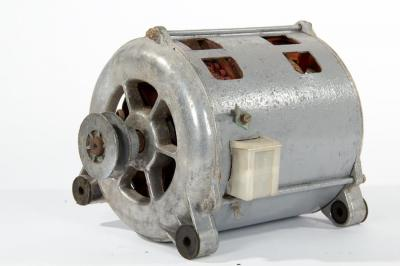
\includegraphics[width=0.37\textwidth]{tech/tools/VyatkaDvig.jpg} 
& 
\noindent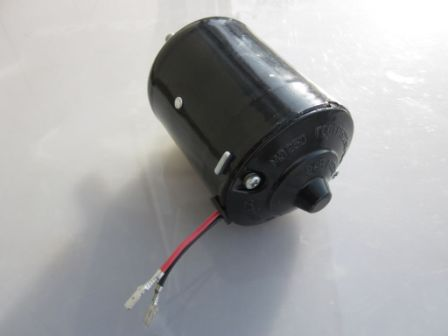
\includegraphics[width=0.37\textwidth]{tech/tools/KamazDvig.jpg}
\\
\textbf{Жвигатель Вятка-Автомат 19??\,г.}
&
\textbf{Двигатель печки Камаза}
\\

\noindent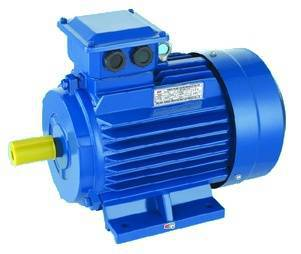
\includegraphics[width=0.37\textwidth]{tech/tools/AIRE.jpg}
& 
\noindent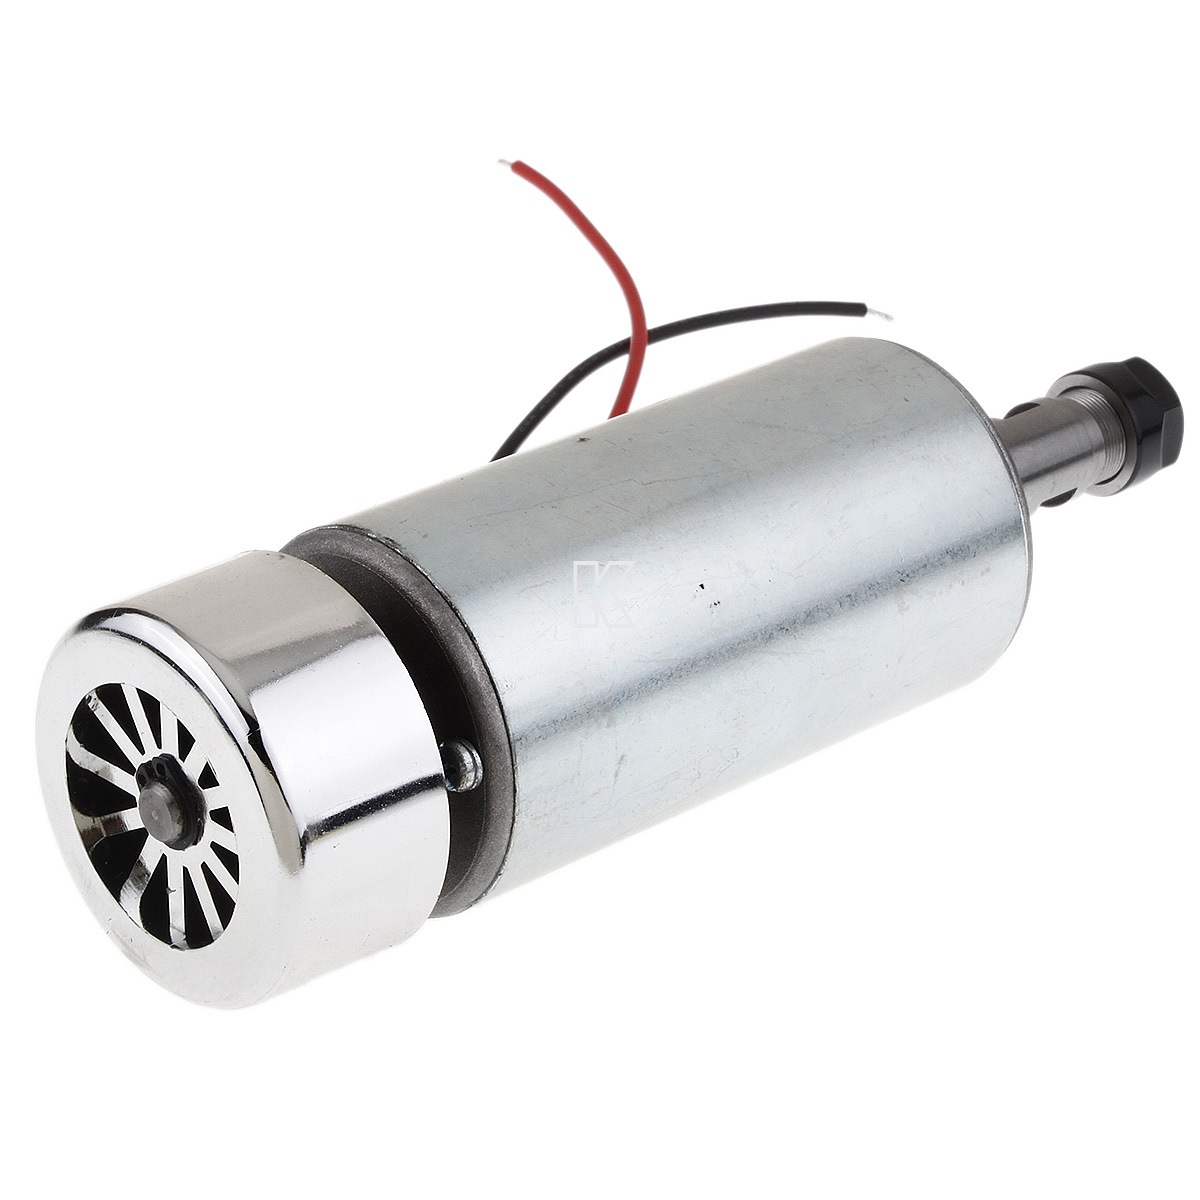
\includegraphics[width=0.37\textwidth]{tech/tools/ER11.jpg}
\\
\textbf{АИРЕ 56 B2, 0.2\,КВт}
&
\textbf{Воздушный шпиндель с цангой ER11}
\\

\end{tabular}
\clearpage

Съемные фрезерные шпиндели, поставляются отдельно или в комплекте с насадкой
ручного фрезера по дереву. Лучшие, со стальной шейкой\ --- Kress, активно
применяются хобби-ЧПУшниками. Попроще и сильно дешевле делал Интерскол, иногда
попадается noname. Недостаток как универсального привода\ --- они
высокоскоростные, возникают проблемы с понижающими передачами. Применение\ ---
приводной высокоскоростной инструмент: боры, фрезы по дереву, микроинструмент
для граверов (микродиски, шарошки). Цанга 8\,мм. Для некоторых моделей бывают
наборы цанг на мелкий инструмент.

\bigskip
\begin{tabular}{p{0.3\textwidth} p{0.3\textwidth} p{0.3\textwidth} }
\noindent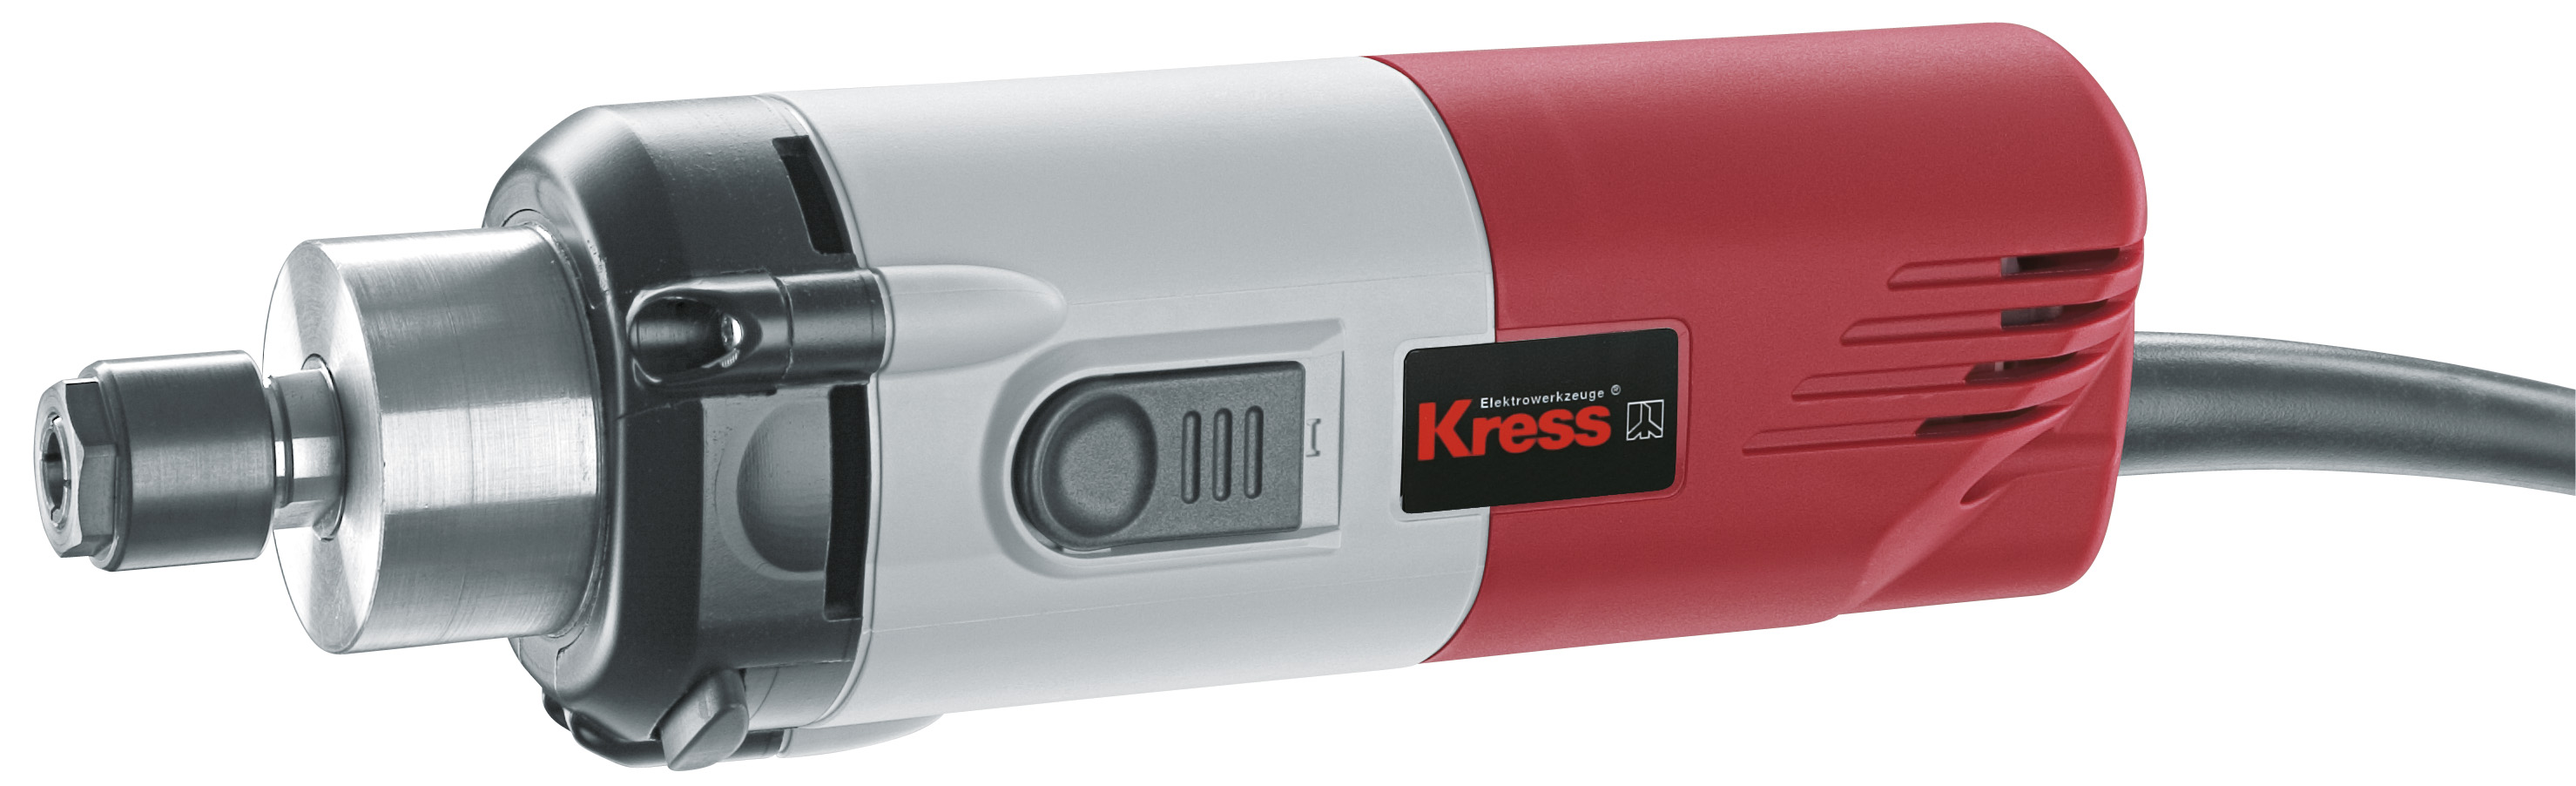
\includegraphics[height=0.3\textheight,width=0.3\textwidth,keepaspectratio]{tech/tools/Kress530.jpg}
&
\noindent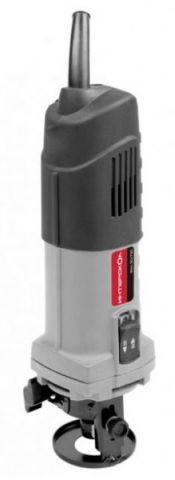
\includegraphics[height=0.3\textheight,width=0.3\textwidth,keepaspectratio]{tech/tools/Interskol30.jpg}
&
\noindent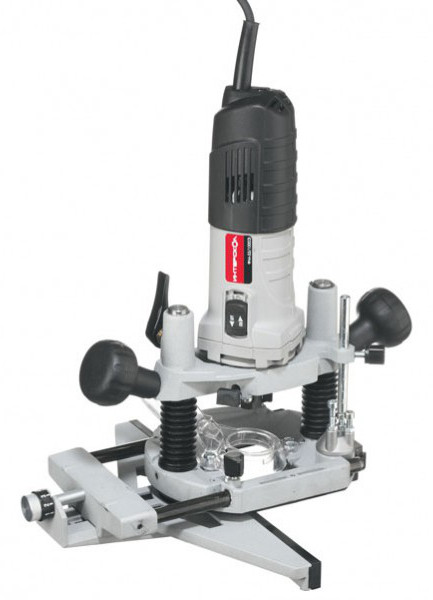
\includegraphics[height=0.3\textheight,width=0.3\textwidth,keepaspectratio]{tech/tools/InterskolFM55.jpg}
\\
KRESS 530/800/1050 FM(E)
&
Интерскол ФМ-30/750
&
Интерскол ФМ-55/1000 Э
\\
\href{http://kress-shop.ru/product/frezernyj-dvigatel-530-fm-kress-06082302/}{5600+\,р.}
&
/снят с производства/
&
\href{http://www.kuvalda.ru/catalog/1867/27920/}{5050\,р.}
\\
\end{tabular}
